%\documentclass[conference]{IEEEtran}
%\IEEEoverridecommandlockouts
\documentclass{article}
\usepackage[utf8]{inputenc}
\usepackage[%
    left=1.0in,%
    right=1.0in,%
    top=1.0in,%
    bottom=1.0in,%
    paperheight=11in,%
    paperwidth=8.5in%
]{geometry}

% =======================
\usepackage{xeCJK}
\usepackage{amssymb}
\usepackage{amsmath}
\usepackage{amstext}
\usepackage{amsopn}
%\usepackage{algorithmic}
\usepackage{graphicx}
\usepackage{textcomp}
\usepackage{xcolor}

\usepackage{textcomp}

\usepackage{boxedminipage}
\usepackage{enumerate}
\usepackage{multirow}
\usepackage{url}
\usepackage{times}
\usepackage{version}
% \usepackage[pdftex]{graphicx}
\usepackage{epsfig}
\usepackage{epsf}
%\usepackage{graphics}
\usepackage{caption}
\usepackage{subfigure}
\usepackage{algorithm}
\usepackage{algpseudocode}
%\PassOptionsToPackage{bookmarks={false}}{hyperref}
%%%%%%%%%%%%
\usepackage{comment}
\usepackage{multicol}
\usepackage{booktabs}
\usepackage{dblfloatfix}
\usepackage{listings}
\usepackage{xparse}
\usepackage{hyperref}
\usepackage{lmodern}
\usepackage{enumitem}
\lstset{language=C,keywordstyle={\bfseries \color{blue}}}

\input macro.tex
% ==========================

\setCJKmainfont[Path=fonts/]{msjh.ttc} % 中文字型
\setCJKmonofont[Path=fonts/]{msjh.ttc} % 中文等寬字型

\begin{document}

\title{E-Healthcare Management System}
\author{
  Cheng-Han Hsieh, 謝承翰\\
  \texttt{B103040012}
  \and
  Shih Yu Sun, 孫世諭\\
  \texttt{B103040001}
  \and
  Casper Liu, 劉世文\\
  \texttt{B093040051}
  \and
  Tina Tsou, 鄒宜庭\\
  \texttt{B096060032}
  \and
  Chia-Yen Huang, 黃嘉彥\\
  \texttt{B103040051}
  \and
  Ting-Hao Hsu, 許廷豪\\
  \texttt{B103040008}
}

\maketitle

\section{Outline}
\label{sec:outline}

  \begin{figure}[h]
    \centering
    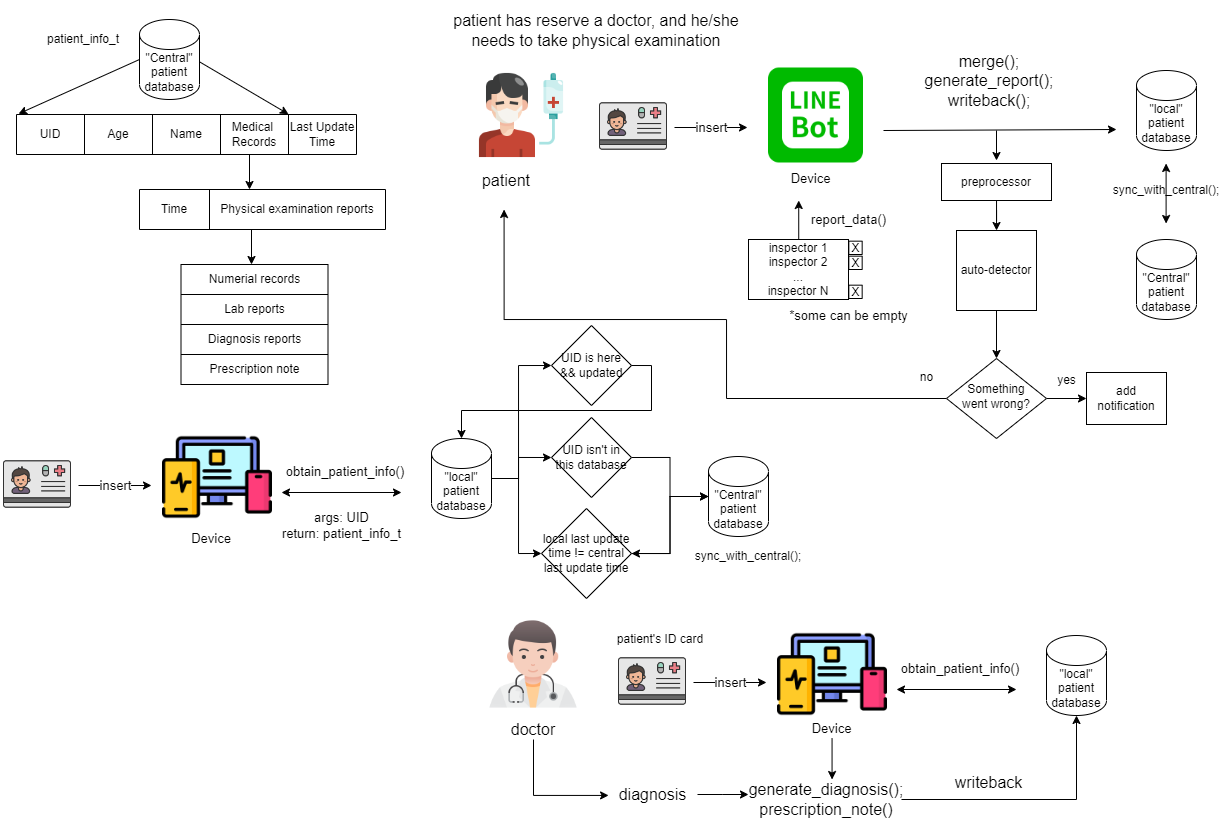
\includegraphics[scale = 0.25]{asset/flowchart.png}
    \caption{A simple example of outline.}
    \label{fig:flowchart}
  \end{figure}

  \xfig{fig:flowchart} shows the skelton of the whole system. The left-top 
  part is the scrawled database, which defines ``what'' is in the database. 
  As shown, the database contains necessary medical information of patients. 
  The right-top part is the situation that a patient has maken an appointment 
  with doctor and he need to take a physical examination first. By insert the 
  ID card, the physical data will be recorded into the local database, syncing 
  with the central database, and in the mean time, the result of examination 
  will be sended to ``auto-detecters'', which detect the abnormal data in the 
  physical reports, and notify the patient. The auto-detecters can detect 
  potential diseases like cancer by determining the gene expression profiling, 
  or diabetes by the physical data. 
  The middle part is the situation that a patient or a doctor wants to obtain 
  the information of the patient. After inserting the ID card, the local 
  database will check whether the status of corresponding data. If it is out of 
  date or not exists, the local database will try to sync with the central 
  database, otherwise create a new one if this patient is totally new. Eventually, 
  the information of this patient is returned to the client (device). 
  The bottom part shows a doctor make the diagnosis and prescription for the 
  patient. The new diagnosis and prescription are write-backed to the local 
  database, and also sync with the central one. 

\section{Features}
\label{sec:features}

  With this E-healthcare management system, the hospital/clinic can easily 
  sync the information of patients with other health systems, manage 
  the information of patients.
  For patients, the patient can do most of the things online, for example, 
  make a doctor appointment, look up the medical records and prescriptions, 
  and obtain the physical reports at home. Even more, the system use machine 
  learning to detect the abnormal data in the reports, notify the patient 
  to prevent the disease becoming worse. 
  To conclusion, the major features of the system can be summarized as 
  followings: 
  \begin{itemize}
    \item Automatically sync the information of patients between different health systems by using local and central database. 
    \item Facilitate the accessing of medical records and prescriptions, for both doctors and patients. 
    \item Introduce the automatic disease detecters by leveraging machine learning and big data. 
  \end{itemize}

\section{Methodology}
\label{sec:methodology}
  \subsection*{Database}
  \begin{figure}[h]
    \centering
    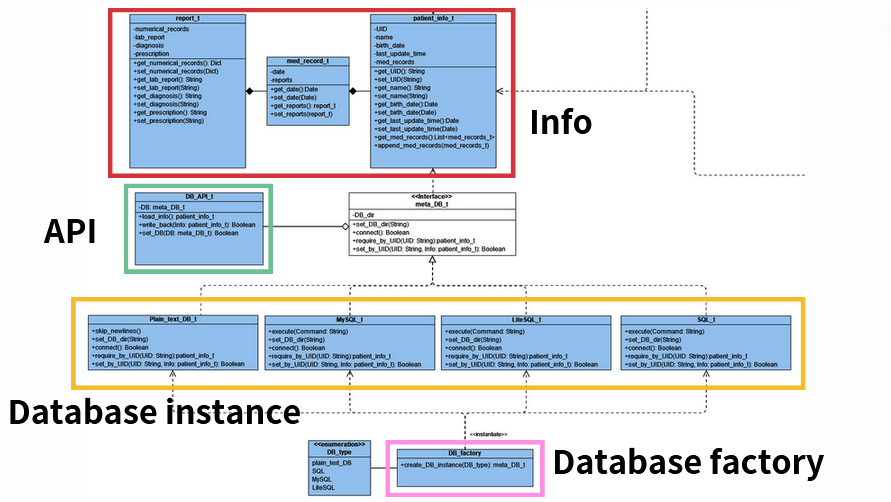
\includegraphics[scale = 0.6]{asset/database/DB_UML.png}
    \caption{The UML of the whole database.}
    \label{fig:DB_UML}
  \end{figure}
  \xfig{fig:DB_UML} shows the UML of the database. It can be divided into four 
  parts, the class definition of patients' information, the database API, the 
  class definition of database, and the database factory. 

  \begin{figure}[h]
    \centering
    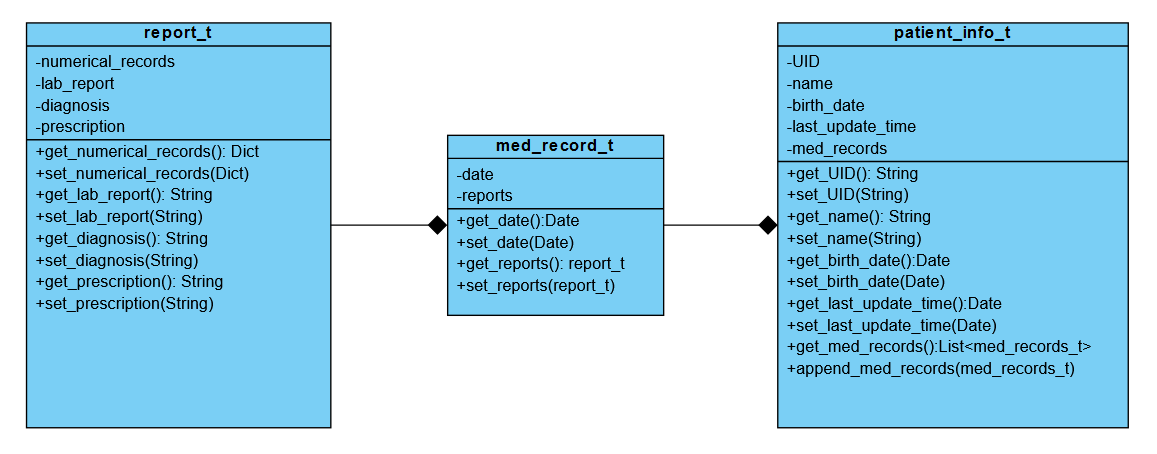
\includegraphics[scale = 0.35]{asset/database/pinfo.png}
    \caption{The UML of the class definition of patient information.}
    \label{fig:pinfo_UML}
  \end{figure}
  \xfig{fig:pinfo_UML} shows the class definition of the patients' information. 
  The class, \codeword{patient\_info\_t}, contains the necessary information of 
  a patient, for example, UID, name, birth date, and the list of medical records. 
  And in the class, \codeword{med\_record\_t}, is date and reports, like diagnosis, 
  prescriptions, and physical data and reports. 
  In this part, it provides a definition of patients' information for the whole 
  database. Later, the database will depend on the class defined in this part. 

  \begin{figure}[h]
    \centering
    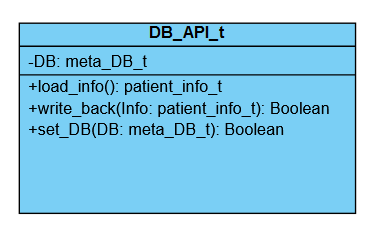
\includegraphics[scale = 0.5]{asset/database/DB_API.png}
    \caption{The UML of the class definition of database API.}
    \label{fig:API_UML}
  \end{figure}
  \xfig{fig:API_UML} is the definition of the API of the database. It provide 
  some simple and secure methods to access the database, for example, load the 
  information of a patient, update the information, and set the database. 
  Later, those parts of the system that need to access the database rely on 
  this API. 

  \begin{figure}[h]
    \centering
    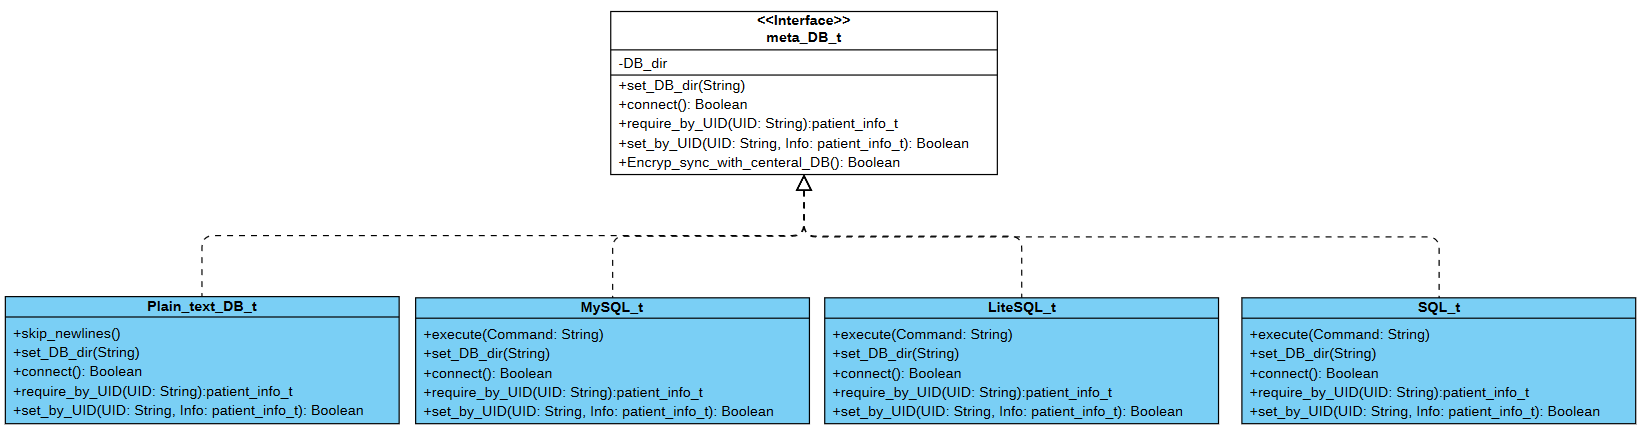
\includegraphics[scale = 0.5]{asset/database/database_instance.png}
    \caption{The UML of the class definition of database instance.}
    \label{fig:DB_instance}
  \end{figure}
  Here is the definition of the databases. First is an interface of the 
  database, it defines some common methods of database, like connect, require, 
  update, and sync with other database. 
  Then are the specialized databases. Here, plain text database, SQLs are defined. 

  The rationales behind the need of an interface is, in the early development, 
  we did not determine which type of database should be use. And second, when 
  scaling the system up, the database may need to be replaced with other databases 
  that have higher throughput and lower response time, like ScyllaDB. 
  An interface of the database solves the problems, because it abstracts the 
  database and unify the methods. The additional databases can be easily provided 
  by following the interface. 

  \begin{figure}[h]
    \centering
    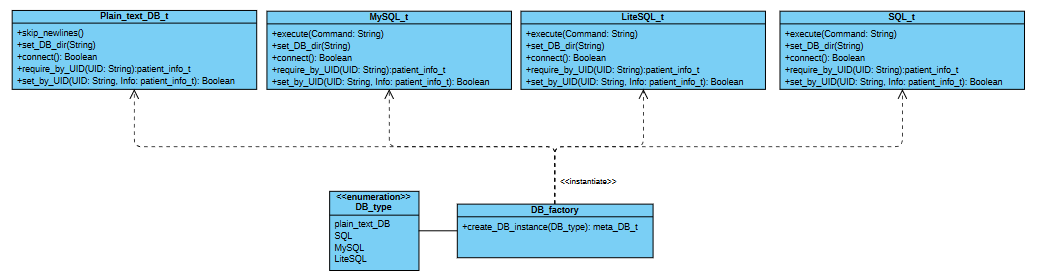
\includegraphics[scale = 0.7]{asset/database/factory_UML.png}
    \caption{The UML of the factory of databases.}
    \label{fig:factory_UML}
  \end{figure}

  \begin{figure}[h]
    \centering
    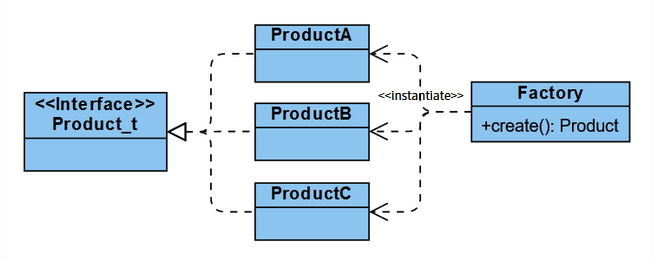
\includegraphics[scale = 0.5]{asset/database/simple_factory.png}
    \caption{The UML of a simple factory.}
    \label{fig:simple_factory}
  \end{figure}
  Then is the factory of database, which shown in \xfig{fig:factory_UML}. 
  In short, factory is responsible for instantiating the database. And it is actually 
  a pattern from $\textit{Design Patterns}$. 
  The general UML of factory pattern is shown in \xfig{fig:simple_factory}. The 
  products inherit a common interface, and they are all instantiated by the factory. 
  The advantage of factory patterns is it hides the details of ``creation'', which 
  allows the factory changing the implementation without modifying the usage of the 
  creation. It is a very import characteristics in developing a big system. The 
  modification of the usage of methods can cost lots of time and effort, because 
  all the programs that use the methods should be modified. 
  
  To conclusion, this design of database has the following features:
  \begin{itemize}
    \item Hide the detail of the creation. 
    \item An uniform application interface. 
    \item High Scalability. 
    \item Easy to maintain. 
  \end{itemize}

%\section{Code}
%\label{sec:code}

\subsection*{Frontend and Medium}

\begin{figure}[h]
  \centering
  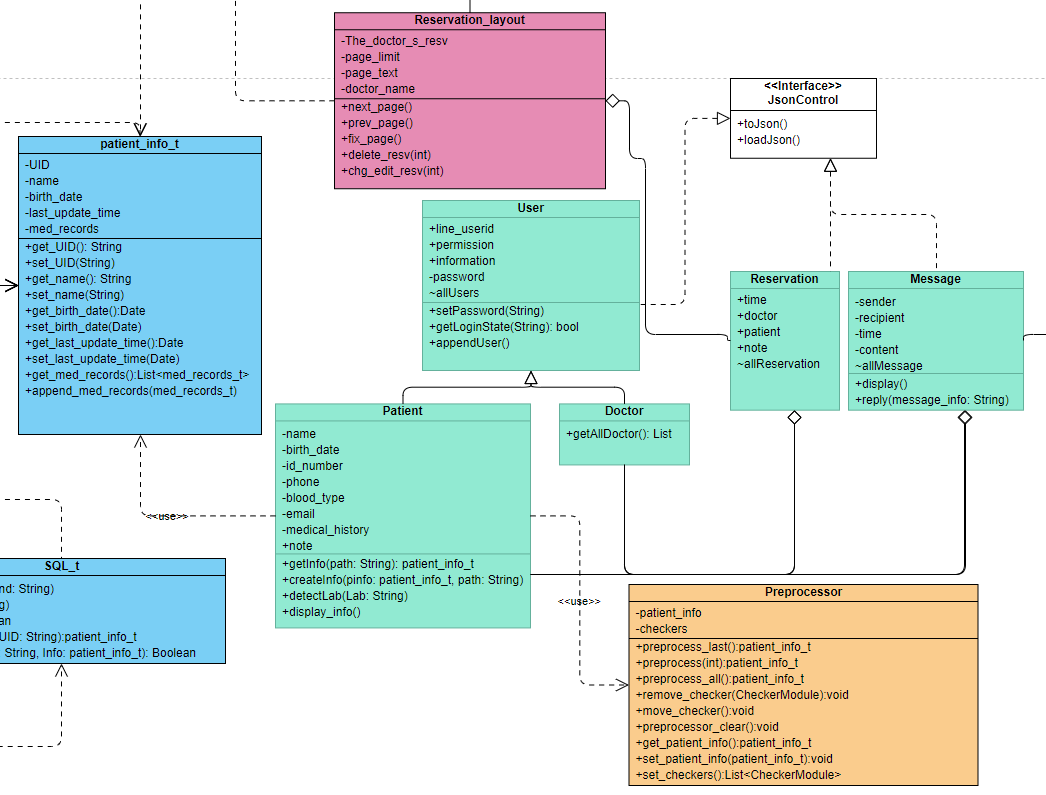
\includegraphics[scale = 0.5]{asset/frontend_and_medium/MED_whole.png}
  \caption{The UML of frontend and medium.}
  \label{fig:uml_frontend_and_medium}
\end{figure}

In the code for the patient frontend and middleware, our functionalities are as follows (refer to Figure \ref{fig:uml_frontend_and_medium}):

\begin{enumerate}[label=\arabic*.]
    \item Utilize Ngrok to forward external requests to the locally specified port.
    \item Integrate LineBot, HTML, JS, and CSS, serving as the patient frontend to send requests such as registration, message sending, and reservations.
    \item Connect to the database to retrieve detailed information based on the user's ID.
    \item Interface with the Processor (Lab), sending detailed information retrieved from the database to the C++ Processor (Lab) for processing and receiving the information back.
    \item Enable the Doctor GUI to utilize the Patient Class to 
    \begin{enumerate}[label=(\roman*)]
        \item obtain detailed information from the database,
        \item access return information from the Processor (Lab),
        \item retrieve the Message Class, and
        \item use the \codeword{Reply()} method to quickly respond to messages via LineBot (refer to Figure \ref{fig:uml_frontend_and_medium}),
        \item obtain detailed data from the Reservation Class,
        \item access the Doctor Class, and
        \item verify its name and password for login.
    \end{enumerate}
\end{enumerate}

Next, we will explain each class in the frontend and medium, highlighting some special member functions and attributes:

\subsubsection*{User}

\begin{itemize}
    \item An abstract class primarily responsible for handling account information such as:
    \begin{enumerate}[label=(\roman*)]
        \item \codeword{permission:} Manages permissions, used to confirm the current user mode (admin or guest).
        \item \codeword{line\_id:} Mainly used to record the user's Line ID, this information is automatically obtained from Line during registration and transmitted to our server.
        \item \codeword{getLoginState(String):} Takes a password as input and checks if it is the correct password.
    \end{enumerate}
\end{itemize}

\subsubsection*{Patient}

\begin{itemize}
    \item A child class of User, mainly deals with patient account information, where it interfaces with the \codeword{patient\_info\_t} in the database to obtain detailed data such as heart rate, blood glucose:
    \begin{enumerate}[label=(\roman*)]
        \item \codeword{detectLab(String):} Will send the information of \codeword{patient\_info\_t} to the Preprocessor, obtaining a detailed diagnosis such as "high heart rate," "diabetes risk," etc (refer to Figure \ref{fig:uml_medium_preprocessor_database}).
    \end{enumerate}
\end{itemize}

\begin{figure}[h]
  \centering
  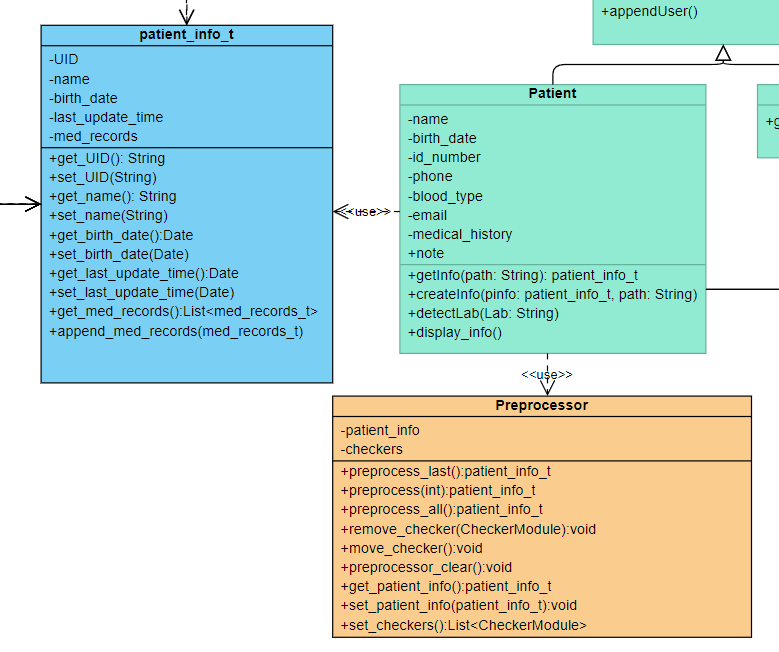
\includegraphics[scale = 0.5]{asset/frontend_and_medium/MED_usage_processor_DB.png}
  \caption{The UML of interaction between medium, preprocessor and database.}
  \label{fig:uml_medium_preprocessor_database}
\end{figure}

\subsubsection*{JsonControl}

\begin{itemize}
    \item An interface implemented by the User, Reservation, and Message classes. Its main purpose is to serialize objects into JSON files for easy storage and access:
    \begin{enumerate}[label=(\roman*)]
        \item \codeword{toJson():} Stores all objects of the entire class in JSON format.
        \item \codeword{loadJson():} Reads a JSON file and restores all objects from it into a list.
    \end{enumerate}
\end{itemize}

\subsubsection*{Reservation}

\begin{itemize}
    \item When a patient uses the frontend LineBot to make a reservation, a Reservation object is created. It is used and deleted by the Doctor GUI and includes Patient and Doctor objects to determine the patient and the reserved doctor (refer to Figure \ref{fig:uml_medium_and_doctor_gui}).
\end{itemize}

\subsubsection*{Message}

\begin{itemize}
    \item When a patient uses the frontend LineBot to send a message, a Message object is created. It is used, replied to, and deleted by the Doctor GUI and includes Patient and Doctor objects to determine the patient and the doctor being messaged (refer to Figure \ref{fig:uml_medium_and_doctor_gui}):
    \begin{enumerate}[label=(\roman*)]
        \item \codeword{reply():} Based on its own Patient object, it uses LineBot to send a message back to the patient (because the Patient object contains the line\_id attribute).
    \end{enumerate}
\end{itemize}

\begin{figure}[h]
  \centering
  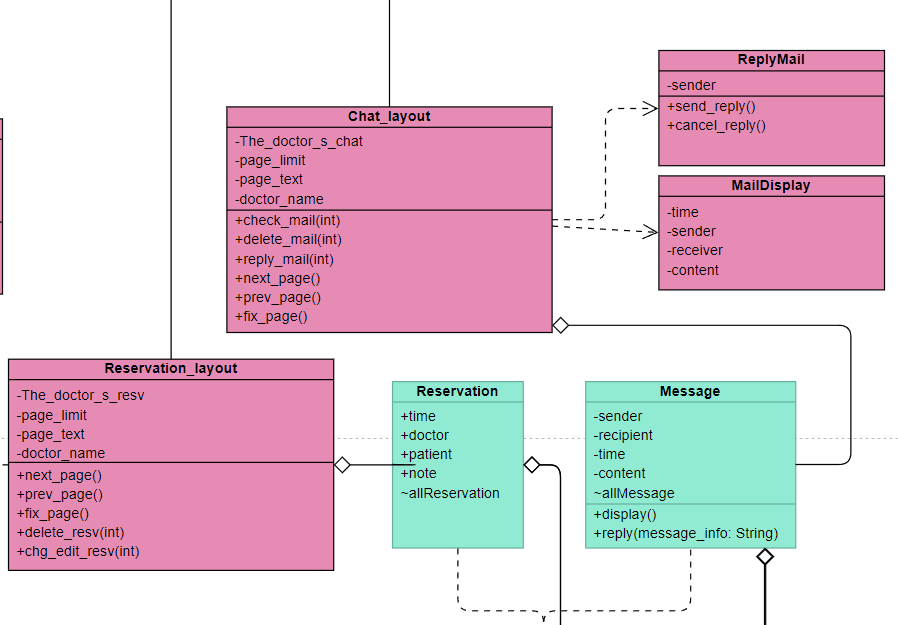
\includegraphics[scale = 0.5]{asset/frontend_and_medium/MED_usage_doctor_gui.png}
  \caption{The UML of interaction between medium and Doctor GUI.}
  \label{fig:uml_medium_and_doctor_gui}
\end{figure}

\section{Conclusion}
\label{sec:conclusion}
In this project, we develope a E-healthcare management system, which solves 
the syncing problem between different health systems by using local and 
central database, and facilitate most of the services by transfer them into 
internet. Even more, we introduce the automatic disease detecters, which 
is able to detect multiple diseases by leveraging the machine learning 
techniques. 

In technological aspect, we use object-oriented programming to shorten the 
development time, and modularize the whole system into several parts, like 
database, frontend, medium, and detecter (processor). With that, the system 
is highly scalable and easy to maintain. 

\section{Contribution}
\label{sec:contribution}

\texttt{B103040012} (Cheng-Han Hsieh, 謝承翰): the design of the whole architecture, database, paper report
\texttt{B103040001} (Shih-Yu Sun, 孫世諭): medium, frontend, linebot, paper report

\end{document}